\documentclass[../main.tex]{subfiles}
\begin{document}
\onlyinsubfile{
\setcounter{chapter}{1}
}
\notinsubfile{}

\subsection*{No cloning theorem -met brakets}
Het is niet mogelijk om een qubit te kopi\"{e}eren, dit is fysisch verboden. In de natuurkunde wordt dit ook wel het 'no cloning theorem' genoemd. Het is best onhandig dat we niet zomaar qubits kunnen kopi\"{e}eren, want dat betekent dat we niet zo makkelijk qubit toestanden kunnen namaken, iets wat we wel graag zouden willen om bijvoorbeeld fouten in een quantumberekening op te sporen (als je drie keer precies dezelfde berekening doet, heb je meer kans dat je op het goede antwoord uitkomt).
Er bestaat een heel kort bewijs voor de no cloning theorem dat we hier zullen bespreken.

Stel, je hebt een qubit operatie die een qubit kan kopi\"{e}eren, bijvoorbeeld de operatie $U$ kan de toestand $\ket{0}$ in een arbitraire toestand $\ket{\psi}$ veranderen, dus:

\begin{equation*}
U\ket{0}\ket{\psi} = \ket{\psi}\ket{\psi}
\end{equation*}

Maar dan zou $U$ ook iedere andere qubit toestand moeten kunnen kopi\"{e}eren, zoals de toestand $\ket{\phi}$:

\begin{equation*}
U\ket{0}\ket{\phi} = \ket{\phi}\ket{\phi}
\end{equation*}

Omdat $U$ een quantumoperatie moet zijn, is $U$ unitair. Als we beide kopieerpogingen met elkaar vermenigvuldigen, krijgen we het volgende:

\begin{equation*}
\bra{\psi}\bra{0}U^*U\ket{0}\ket{\phi} = \bra{\psi}\bra{\psi}\ket{\phi}\ket{\phi}
\end{equation*}

We weten dat een in product van een object met zichzelf $1$ is, dus $\bra{0}\ket{0}=1$ en $U^*U=1$, dus we krijgen:

\begin{equation*}
|\bra{\psi}\ket{\phi}| = |\bra{\psi}\ket{\phi}\bra{\psi}\ket{\phi}| = |\bra{\psi}\ket{\phi}|^2
\end{equation*}

Deze formule klopt alleen als $|\bra{\psi}\ket{\phi}| = 1$ of als $|\bra{\psi}\ket{\phi}| = 0$, dus als ofwel $\phi=\psi$, ofwel $\phi$ staat loodrecht op $\psi$. Maar we hadden $\phi$ en $\psi$ als twee random toestanden gekozen. Een operatie $U$ kan dus geen \textit{algemene} quantumtoestand kopi\"{e}ren.

\clearpage

\section*{No cloning theorem too}
\marginpar{\nogdoen{No cloning staat in de bolletjes bij H2, lineariteit wordt pas in H3 behandeld. opl: noem in H2, verwijs naar H3, daar ook het bewijs (ruim een pagina}}
Het is niet mogelijk een qubit te kopi\"eren. Dit staat bekend als het 'no-cloning theorema'. We geven een bewijs uit het ongerijmde. In zo'n bewijs probeer je eerst aan te tonen dat de stelling geldt, daarna laat je zien dat dat een foute aanname is, waarna je moet concluderen dat de stelling ongeldig is.

Om te kopi\"eren hebben we een mal nodig. We nemen daarvoor de basistoestanen $\ket{0}$ en $\ket{1}$. Met de regels van lineariteit kunnen we dan ook een willekeurige toestand  $\ket{\Psi}$ uitrekenen. Je moet ook iets in de mal 'gieten'. Dat kan een basistoestand zijn. We nemen daarvoor $\ket{0}$.

%We nemen aan dat er een poort \port{U} is die toestand $\ket{\Psi}$ kan kopi\"eren:
%\[\begin{aligned}\label{eq:copy}
%\port{U}\ket{\Psi}\ket{0}=\ket{\Psi}\ket{\Psi}
%\end{aligned}\]

We zetten de twee qubits in \'e\'en ket. De \port{U}-poort kopieert het linker qubit.
\[\begin{aligned} \port{U}\ket{00} = \ket{00} \quad \mathrm{en} \quad \port{U}\ket{10}=\ket{11}
\end{aligned}\]

Vraag A: Stel de operatie op die toestand $\ket{\Psi}$ kopieert.\\
\begin{antwoord}
$U\ket{0\psi} = \ket{\psi\psi}$
\end{antwoord}

De twee operaties mogen we samenvoegen (in superpositie brengen). We passen daarbij de regels van lineariteit toe (\nogdoen{ref}):
\[\begin{aligned}\port{U}(\tfrac{1}{\sqrt{2}}(\ket{00}+\ket{10}))=\tfrac{1}{\sqrt{2}}(\port{U}\ket{00}+\port{U}\ket{10})=
\tfrac{1}{\sqrt{2}}((\ket{00}+\ket{11})\end{aligned}\]
Je moet tot hetzelfde resultaat komen als je $\ket{0}$ in de begintoestand  buiten haakjes haalt:
%\begin{align}
%\frac{\ket{00}+\ket{10}}{\sqrt{2}}=\frac{\ket{0}+\ket{1}}{\sqrt{2}}\ket{0}
%\end{align}
\[\begin{aligned}
\port{U}\bigg(\frac{\ket{00}+\ket{10}}{\sqrt{2}}\bigg)&=
\port{U}\bigg(\frac{\ket{0}+\ket{1}}{\sqrt{2}}\ket{0}\bigg) = \\
%&\stackrel{\text{pas vgl.~\ref{eq:copy} toe}}{=}\\
\bigg(\frac{\ket{0}+\ket{1}}{\sqrt{2}}\bigg)\bigg(\frac{\ket{0}+\ket{1}}{\sqrt{2}}\bigg)&=\frac{1}{2}(\ket{00}+\ket{01}+\ket{10}+\ket{11})\\
&\neq \frac{1}{\sqrt{2}}((\ket{00}+\ket{11})
\end{aligned}\]

Vraag B: Geef het no-cloning bewijs met $\ket{1}$ als mal.

Vraag C: Waarom geldt het no-cloning theorema voor een willekeurige toetstand $\ket{\Psi}$?


\section*{No cloning theorem ronald}
Stel dat je een \nogdoen{unitaire 2-qubit} operatie \port{U} hebt die een qubit kan clonen (dat wil zeggen een kopie van het eerste qubit kan maken in het tweede qubit, dat begint in toestand $\ket{0}$). Omdat U in ieder geval de twee basistoestanden $\ket{0}$ en $\ket{1}$ moet kunnen clonen, heb je:
\[\beginaligned}
 U\ket{0}\ket{0} &=\ket{0}\ket{0}\\
 U\ket{1}\ket{0} &=\ket{1}\ket{1}
\end{aligned}\]

Stel nu dat je probeert een qubit in toestand $\ket{+} =1/sqrt{2}(\ket{0} +\ket{1}$ ) te clonen.
 We hebben:

 $U\ket{+}\ket{0} =1/sqrt{2}(U\ket{0}\ket{0} +U\ket{1}\ket{0})=1/sqrt{2}(\ket{0}\ket{0} +\ket{1}\ket{1})$, wegens lineariteit. Die laatste toestand is een EPR-paar, dus entangled, dus kan niet gelijk zijn aan de toestand $\ket{+}\ket{+}$ die de cloner had moeten maken. De aanname dat zo'n U bestaat leidt dus tot een tegenspraak, QED.


\section*{No cloning theorem Guido}


Waarom is cloning bij qubits niet mogelijk?
Het antwoord heeft te maken met het feit dat een quantum-operator reversibel moet zijn.
Bekijk onderstaande afbeelding.


\begin{flushleft}
\begin{minipage}{.45\textwidth}
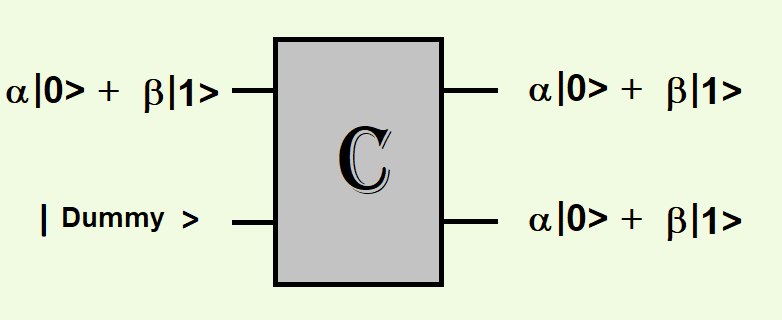
\includegraphics[width=\textwidth]{./img/nocloning.png}
\end{minipage}%
\hfill
\begin{minipage}{.5\textwidth}
 \captionof{figure}{schema waarmee je  een qubit zou kunnen  clonen}. \label {fig:nocloning}
\end{minipage}%
\end{flushleft}


\marginpar{\nogdoen{Deze oplossing past overal, simpelheid zelve}}

Cloning houdt in dat de toestand van een qubit wordt gedupliceerd. Een tweede qubit moet dus de toestand van de te clonen qubit overnemen. 
De werking van een poort is bekend als de werking bekend is op de basistoestanden.
Er zijn vier verschillende combinaties van de input mogelijk. In de tabel hieronder  is weergegeven wat de output is bij deze vier combinaties.


\begin{flushleft}
\begin{minipage}{.25\textwidth}
%\begin{table}[]
\begin{tabular}{|c||c|}
\hline
 $in$  & $out$  \\ \hline
 00    & 00     \\ \hline
 01    & 00     \\ \hline
 10    & 11     \\ \hline
 11    & 11     \\ \hline
\end{tabular}
%\end{table}
\end{minipage}%
\hfill
\begin{minipage}{.7\textwidth}
\captionof{figure}{Aan de tabel is te zien dat de werking van de poort niet ongedaan kan worden gemaakt. Er gaat door de werking van de poort informatie verloren. De poort is niet reversibel. Een quantumpoort die een qubit cloont bestaat dus niet.\label{fig:viermogelijkheden}}
\end{minipage}
\end{flushleft}



\end{document}
